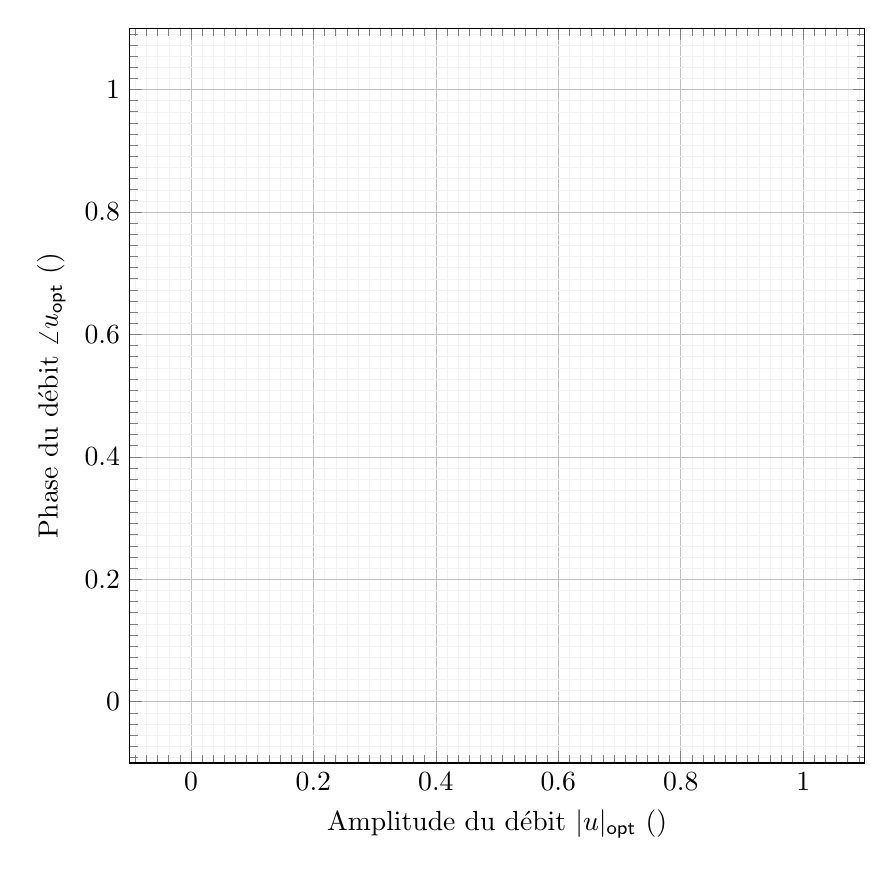
\begin{tikzpicture}
    \def\width{.9*\textwidth};
    \def\height{\width};
    \def\spx{.25cm};
    \def\spy{1.25cm};
    \def\legx{.5cm};
    \def\legy{\legx};
    \def\prop{.45};
 
    
    \begin{axis}[width={\width},height={\height},
    grid=both, minor tick num=10, 
    grid style={line width=.1pt, draw=gray!10},
    major grid style={line width=.2pt,draw=gray!50},
    xlabel={Amplitude du débit $|u|_{\sf opt}$ (\unit{\cubic\meter\per\second})},
    ylabel={Phase du débit $\angle u_{\sf opt}$ (\unit{\cubic\meter\per\second})},
%    xmin=0,xmax=75,ymin=0,ymax=.5/1000,
%    xtick={0,25,50,75,100},
%    ytick={0,1e-4,...,10e-4},
%    ytick={0,2.81/100000,9.1120/100000,1.4452/10000,
%    	2.5/10000,5/10000,1/1000},
    scaled y ticks = false,
    domain=0:100,
    legend cell align={left},
    legend style = {at={($(1,1)+(-2mm,-2mm)$)},anchor = north east,rounded corners}
    ]
        
    \end{axis}
\end{tikzpicture}